% Options for packages loaded elsewhere
\PassOptionsToPackage{unicode}{hyperref}
\PassOptionsToPackage{hyphens}{url}
%
\documentclass[
]{article}
\usepackage{amsmath,amssymb}
\usepackage{lmodern}
\usepackage{iftex}
\ifPDFTeX
  \usepackage[T1]{fontenc}
  \usepackage[utf8]{inputenc}
  \usepackage{textcomp} % provide euro and other symbols
\else % if luatex or xetex
  \usepackage{unicode-math}
  \defaultfontfeatures{Scale=MatchLowercase}
  \defaultfontfeatures[\rmfamily]{Ligatures=TeX,Scale=1}
\fi
% Use upquote if available, for straight quotes in verbatim environments
\IfFileExists{upquote.sty}{\usepackage{upquote}}{}
\IfFileExists{microtype.sty}{% use microtype if available
  \usepackage[]{microtype}
  \UseMicrotypeSet[protrusion]{basicmath} % disable protrusion for tt fonts
}{}
\makeatletter
\@ifundefined{KOMAClassName}{% if non-KOMA class
  \IfFileExists{parskip.sty}{%
    \usepackage{parskip}
  }{% else
    \setlength{\parindent}{0pt}
    \setlength{\parskip}{6pt plus 2pt minus 1pt}}
}{% if KOMA class
  \KOMAoptions{parskip=half}}
\makeatother
\usepackage{xcolor}
\usepackage[margin=1in]{geometry}
\usepackage{color}
\usepackage{fancyvrb}
\newcommand{\VerbBar}{|}
\newcommand{\VERB}{\Verb[commandchars=\\\{\}]}
\DefineVerbatimEnvironment{Highlighting}{Verbatim}{commandchars=\\\{\}}
% Add ',fontsize=\small' for more characters per line
\usepackage{framed}
\definecolor{shadecolor}{RGB}{248,248,248}
\newenvironment{Shaded}{\begin{snugshade}}{\end{snugshade}}
\newcommand{\AlertTok}[1]{\textcolor[rgb]{0.94,0.16,0.16}{#1}}
\newcommand{\AnnotationTok}[1]{\textcolor[rgb]{0.56,0.35,0.01}{\textbf{\textit{#1}}}}
\newcommand{\AttributeTok}[1]{\textcolor[rgb]{0.77,0.63,0.00}{#1}}
\newcommand{\BaseNTok}[1]{\textcolor[rgb]{0.00,0.00,0.81}{#1}}
\newcommand{\BuiltInTok}[1]{#1}
\newcommand{\CharTok}[1]{\textcolor[rgb]{0.31,0.60,0.02}{#1}}
\newcommand{\CommentTok}[1]{\textcolor[rgb]{0.56,0.35,0.01}{\textit{#1}}}
\newcommand{\CommentVarTok}[1]{\textcolor[rgb]{0.56,0.35,0.01}{\textbf{\textit{#1}}}}
\newcommand{\ConstantTok}[1]{\textcolor[rgb]{0.00,0.00,0.00}{#1}}
\newcommand{\ControlFlowTok}[1]{\textcolor[rgb]{0.13,0.29,0.53}{\textbf{#1}}}
\newcommand{\DataTypeTok}[1]{\textcolor[rgb]{0.13,0.29,0.53}{#1}}
\newcommand{\DecValTok}[1]{\textcolor[rgb]{0.00,0.00,0.81}{#1}}
\newcommand{\DocumentationTok}[1]{\textcolor[rgb]{0.56,0.35,0.01}{\textbf{\textit{#1}}}}
\newcommand{\ErrorTok}[1]{\textcolor[rgb]{0.64,0.00,0.00}{\textbf{#1}}}
\newcommand{\ExtensionTok}[1]{#1}
\newcommand{\FloatTok}[1]{\textcolor[rgb]{0.00,0.00,0.81}{#1}}
\newcommand{\FunctionTok}[1]{\textcolor[rgb]{0.00,0.00,0.00}{#1}}
\newcommand{\ImportTok}[1]{#1}
\newcommand{\InformationTok}[1]{\textcolor[rgb]{0.56,0.35,0.01}{\textbf{\textit{#1}}}}
\newcommand{\KeywordTok}[1]{\textcolor[rgb]{0.13,0.29,0.53}{\textbf{#1}}}
\newcommand{\NormalTok}[1]{#1}
\newcommand{\OperatorTok}[1]{\textcolor[rgb]{0.81,0.36,0.00}{\textbf{#1}}}
\newcommand{\OtherTok}[1]{\textcolor[rgb]{0.56,0.35,0.01}{#1}}
\newcommand{\PreprocessorTok}[1]{\textcolor[rgb]{0.56,0.35,0.01}{\textit{#1}}}
\newcommand{\RegionMarkerTok}[1]{#1}
\newcommand{\SpecialCharTok}[1]{\textcolor[rgb]{0.00,0.00,0.00}{#1}}
\newcommand{\SpecialStringTok}[1]{\textcolor[rgb]{0.31,0.60,0.02}{#1}}
\newcommand{\StringTok}[1]{\textcolor[rgb]{0.31,0.60,0.02}{#1}}
\newcommand{\VariableTok}[1]{\textcolor[rgb]{0.00,0.00,0.00}{#1}}
\newcommand{\VerbatimStringTok}[1]{\textcolor[rgb]{0.31,0.60,0.02}{#1}}
\newcommand{\WarningTok}[1]{\textcolor[rgb]{0.56,0.35,0.01}{\textbf{\textit{#1}}}}
\usepackage{longtable,booktabs,array}
\usepackage{calc} % for calculating minipage widths
% Correct order of tables after \paragraph or \subparagraph
\usepackage{etoolbox}
\makeatletter
\patchcmd\longtable{\par}{\if@noskipsec\mbox{}\fi\par}{}{}
\makeatother
% Allow footnotes in longtable head/foot
\IfFileExists{footnotehyper.sty}{\usepackage{footnotehyper}}{\usepackage{footnote}}
\makesavenoteenv{longtable}
\usepackage{graphicx}
\makeatletter
\def\maxwidth{\ifdim\Gin@nat@width>\linewidth\linewidth\else\Gin@nat@width\fi}
\def\maxheight{\ifdim\Gin@nat@height>\textheight\textheight\else\Gin@nat@height\fi}
\makeatother
% Scale images if necessary, so that they will not overflow the page
% margins by default, and it is still possible to overwrite the defaults
% using explicit options in \includegraphics[width, height, ...]{}
\setkeys{Gin}{width=\maxwidth,height=\maxheight,keepaspectratio}
% Set default figure placement to htbp
\makeatletter
\def\fps@figure{htbp}
\makeatother
\setlength{\emergencystretch}{3em} % prevent overfull lines
\providecommand{\tightlist}{%
  \setlength{\itemsep}{0pt}\setlength{\parskip}{0pt}}
\setcounter{secnumdepth}{-\maxdimen} % remove section numbering
\ifLuaTeX
  \usepackage{selnolig}  % disable illegal ligatures
\fi
\IfFileExists{bookmark.sty}{\usepackage{bookmark}}{\usepackage{hyperref}}
\IfFileExists{xurl.sty}{\usepackage{xurl}}{} % add URL line breaks if available
\urlstyle{same} % disable monospaced font for URLs
\hypersetup{
  pdftitle={Métodos Multivariados: Tarea 1},
  pdfauthor={Aldo, Diego, Mateo, Victor},
  hidelinks,
  pdfcreator={LaTeX via pandoc}}

\title{Métodos Multivariados: Tarea 1}
\author{Aldo, Diego, Mateo, Victor}
\date{31/01/2024}

\begin{document}
\maketitle

\begin{Shaded}
\begin{Highlighting}[]
\FunctionTok{library}\NormalTok{(dplyr)}
\end{Highlighting}
\end{Shaded}

\begin{verbatim}

Attaching package: 'dplyr'
\end{verbatim}

\begin{verbatim}
The following objects are masked from 'package:stats':

    filter, lag
\end{verbatim}

\begin{verbatim}
The following objects are masked from 'package:base':

    intersect, setdiff, setequal, union
\end{verbatim}

\begin{Shaded}
\begin{Highlighting}[]
\FunctionTok{library}\NormalTok{(lattice)}
\FunctionTok{library}\NormalTok{(tidyverse)}
\end{Highlighting}
\end{Shaded}

\begin{verbatim}
-- Attaching core tidyverse packages -------------------------------------------- tidyverse 2.0.0 --
v forcats   1.0.0     v readr     2.1.4
v ggplot2   3.4.4     v stringr   1.5.0
v lubridate 1.9.2     v tibble    3.2.1
v purrr     1.0.1     v tidyr     1.3.0
\end{verbatim}

\begin{verbatim}
-- Conflicts -------------------------------------------------------------- tidyverse_conflicts() --
x dplyr::filter() masks stats::filter()
x dplyr::lag()    masks stats::lag()
i Use the ]8;;http://conflicted.r-lib.org/conflicted package]8;; to force all conflicts to become errors
\end{verbatim}

\begin{Shaded}
\begin{Highlighting}[]
\FunctionTok{library}\NormalTok{(ggplot2)}
\FunctionTok{library}\NormalTok{(ggExtra)}
\FunctionTok{library}\NormalTok{(plotly)}
\end{Highlighting}
\end{Shaded}

\begin{verbatim}

Attaching package: 'plotly'

The following object is masked from 'package:ggplot2':

    last_plot

The following object is masked from 'package:stats':

    filter

The following object is masked from 'package:graphics':

    layout
\end{verbatim}

\begin{Shaded}
\begin{Highlighting}[]
\FunctionTok{library}\NormalTok{(aplpack)}
\FunctionTok{library}\NormalTok{(pander)}
\end{Highlighting}
\end{Shaded}

\hypertarget{ejercicio-1.2}{%
\section{Ejercicio 1.2)}\label{ejercicio-1.2}}

\hypertarget{a}{%
\subsection{a)}\label{a}}

scatterplot A morning newspaper lists the following used-car prices for
a foreign compact with age \(x_i\) measurred in years and selling price
\(x_2\) measurred in thousands of dollars.

\begin{Shaded}
\begin{Highlighting}[]
\NormalTok{x1 }\OtherTok{\textless{}{-}} \FunctionTok{c}\NormalTok{(}\DecValTok{1}\NormalTok{, }\DecValTok{2}\NormalTok{, }\DecValTok{3}\NormalTok{, }\DecValTok{3}\NormalTok{, }\DecValTok{4}\NormalTok{, }\DecValTok{5}\NormalTok{, }\DecValTok{6}\NormalTok{, }\DecValTok{8}\NormalTok{, }\DecValTok{9}\NormalTok{, }\DecValTok{11}\NormalTok{)}
\NormalTok{x2 }\OtherTok{\textless{}{-}} \FunctionTok{c}\NormalTok{(}\FloatTok{18.95}\NormalTok{, }\DecValTok{19}\NormalTok{, }\FloatTok{17.95}\NormalTok{, }\FloatTok{15.54}\NormalTok{, }\DecValTok{14}\NormalTok{, }\FloatTok{12.95}\NormalTok{, }\FloatTok{8.94}\NormalTok{, }\FloatTok{7.49}\NormalTok{, }\DecValTok{6}\NormalTok{, }\FloatTok{3.99}\NormalTok{)}
\NormalTok{datos }\OtherTok{\textless{}{-}} \FunctionTok{data.frame}\NormalTok{(x1, x2)}

\NormalTok{(plot }\OtherTok{\textless{}{-}} \FunctionTok{ggplot}\NormalTok{(datos, }\FunctionTok{aes}\NormalTok{(x1, x2)) }\SpecialCharTok{+} \FunctionTok{geom\_point}\NormalTok{())}
\end{Highlighting}
\end{Shaded}

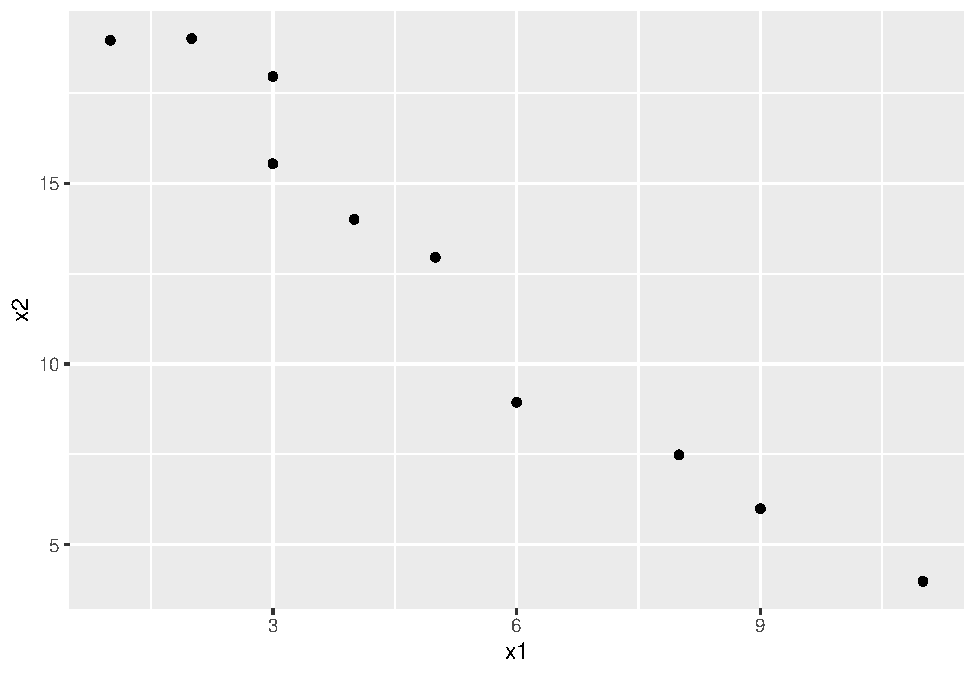
\includegraphics{Tarea1_files/figure-latex/unnamed-chunk-3-1.pdf}

marginal dot diagram

\begin{Shaded}
\begin{Highlighting}[]
\NormalTok{plot1 }\OtherTok{\textless{}{-}} \FunctionTok{ggMarginal}\NormalTok{(plot, }\AttributeTok{type=}\StringTok{"histogram"}\NormalTok{)}
\NormalTok{plot2 }\OtherTok{\textless{}{-}} \FunctionTok{ggMarginal}\NormalTok{(plot, }\AttributeTok{type=}\StringTok{"boxplot"}\NormalTok{)}
\NormalTok{plot3 }\OtherTok{\textless{}{-}} \FunctionTok{ggMarginal}\NormalTok{(plot, }\AttributeTok{type=}\StringTok{"density"}\NormalTok{)}

\NormalTok{plot1}
\NormalTok{plot2}
\NormalTok{plot3}
\end{Highlighting}
\end{Shaded}

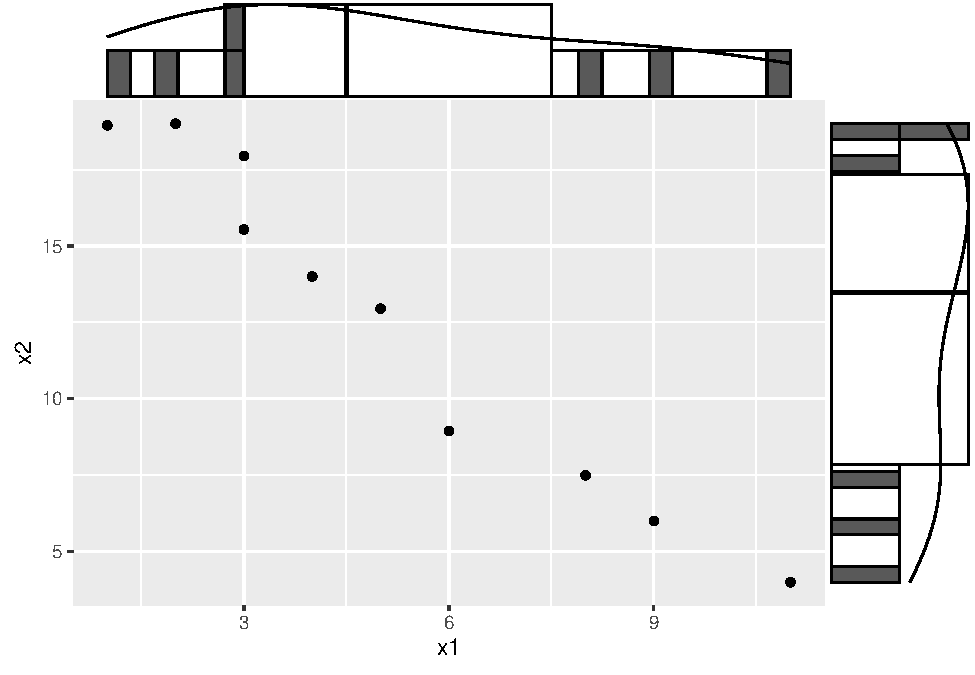
\includegraphics{Tarea1_files/figure-latex/unnamed-chunk-4-1.pdf}

\hypertarget{b}{%
\subsection{b)}\label{b}}

Infiero que la covarianza es negativa porque hay una tendencia: entre
más años tiene el carro, en menos precio se vende.

\hypertarget{c}{%
\subsection{c)}\label{c}}

\begin{Shaded}
\begin{Highlighting}[]
\NormalTok{m1 }\OtherTok{\textless{}{-}} \FunctionTok{mean}\NormalTok{(x1)}
\NormalTok{m2 }\OtherTok{\textless{}{-}} \FunctionTok{mean}\NormalTok{(x2)}

\NormalTok{s11 }\OtherTok{\textless{}{-}} \FunctionTok{var}\NormalTok{(x1)}
\NormalTok{s22 }\OtherTok{\textless{}{-}} \FunctionTok{var}\NormalTok{(x2)}

\NormalTok{s12 }\OtherTok{\textless{}{-}} \FunctionTok{cov}\NormalTok{(x1, x2)}
\NormalTok{r12 }\OtherTok{\textless{}{-}} \FunctionTok{cor}\NormalTok{(x1, x2)}

\FunctionTok{cat}\NormalTok{(}\StringTok{"media x1: "}\NormalTok{, m1, }\StringTok{"}\SpecialCharTok{\textbackslash{}n}\StringTok{"}\NormalTok{, }
       \StringTok{"media x2: "}\NormalTok{, m2, }\StringTok{"}\SpecialCharTok{\textbackslash{}n}\StringTok{"}\NormalTok{,}
       \StringTok{"varianza x1: "}\NormalTok{, s11, }\StringTok{"}\SpecialCharTok{\textbackslash{}n}\StringTok{"}\NormalTok{,}
       \StringTok{"varianza x2: "}\NormalTok{, s22, }\StringTok{"}\SpecialCharTok{\textbackslash{}n}\StringTok{"}\NormalTok{,}
       \StringTok{"covarianza: "}\NormalTok{, s12, }\StringTok{"}\SpecialCharTok{\textbackslash{}n}\StringTok{"}\NormalTok{,}
       \StringTok{"correlación: "}\NormalTok{, r12, }\StringTok{"}\SpecialCharTok{\textbackslash{}n}\StringTok{"}\NormalTok{)}
\end{Highlighting}
\end{Shaded}

\begin{verbatim}
media x1:  5.2 
 media x2:  12.481 
 varianza x1:  10.62222 
 varianza x2:  30.85437 
 covarianza:  -17.71022 
 correlación:  -0.9782684 
\end{verbatim}

Interpretación:

Media x1: 5.2 años. Representa el valor central de los años de
antigüedad de los autos.

Media x2: \$12,481. Indica el valor central de los precios de los autos.

Varianza x1: 10.62222. Refleja la dispersión de los años de antigüedad
de los autos alrededor de su valor central.

Varianza x2: 30.85437. Muestra la dispersión de los precios de los autos
alrededor de su valor central.

Covarianza: -17.71022. Indica cómo varían conjuntamente los años de
antigüedad y los precios de los autos. Una covarianza negativa sugiere
que los autos más antiguos tienden a tener precios más bajos, y
viceversa.

Correlación: -0.9782684. Representa la fuerza y la dirección de la
relación entre los años de antigüedad y los precios de los autos. Una
correlación negativa cercana a -1 indica una fuerte relación inversa: a
medida que los años de antigüedad aumentan, los precios tienden a
disminuir

\hypertarget{d}{%
\subsection{d)}\label{d}}

\begin{Shaded}
\begin{Highlighting}[]
\FunctionTok{colMeans}\NormalTok{(datos)}
\end{Highlighting}
\end{Shaded}

\begin{verbatim}
    x1     x2 
 5.200 12.481 
\end{verbatim}

\begin{Shaded}
\begin{Highlighting}[]
\FunctionTok{var}\NormalTok{(datos)}
\end{Highlighting}
\end{Shaded}

\begin{verbatim}
          x1        x2
x1  10.62222 -17.71022
x2 -17.71022  30.85437
\end{verbatim}

\begin{Shaded}
\begin{Highlighting}[]
\FunctionTok{cor}\NormalTok{(datos)}
\end{Highlighting}
\end{Shaded}

\begin{verbatim}
           x1         x2
x1  1.0000000 -0.9782684
x2 -0.9782684  1.0000000
\end{verbatim}

\hypertarget{ejercicio-1.4}{%
\section{Ejercicio 1.4)}\label{ejercicio-1.4}}

\hypertarget{a-1}{%
\subsection{a)}\label{a-1}}

\begin{Shaded}
\begin{Highlighting}[]
\NormalTok{df }\OtherTok{\textless{}{-}} \FunctionTok{data.frame}\NormalTok{(}
  \AttributeTok{x1 =} \FunctionTok{c}\NormalTok{(}\FloatTok{108.28}\NormalTok{, }\FloatTok{152.36}\NormalTok{, }\FloatTok{95.04}\NormalTok{, }\FloatTok{65.45}\NormalTok{, }\FloatTok{62.97}\NormalTok{, }\FloatTok{263.99}\NormalTok{, }\FloatTok{265.19}\NormalTok{, }\FloatTok{285.06}\NormalTok{, }\FloatTok{92.01}\NormalTok{, }\FloatTok{165.68}\NormalTok{),}
  \AttributeTok{x2 =} \FunctionTok{c}\NormalTok{(}\FloatTok{17.05}\NormalTok{, }\FloatTok{16.59}\NormalTok{, }\FloatTok{10.91}\NormalTok{, }\FloatTok{14.14}\NormalTok{, }\FloatTok{9.52}\NormalTok{, }\FloatTok{25.33}\NormalTok{, }\FloatTok{18.54}\NormalTok{, }\FloatTok{15.73}\NormalTok{, }\FloatTok{8.10}\NormalTok{, }\FloatTok{11.13}\NormalTok{),}
  \AttributeTok{x3 =} \FunctionTok{c}\NormalTok{(}\FloatTok{1484.10}\NormalTok{, }\FloatTok{750.33}\NormalTok{, }\FloatTok{766.42}\NormalTok{, }\FloatTok{1110.46}\NormalTok{, }\FloatTok{1031.29}\NormalTok{, }\FloatTok{195.26}\NormalTok{, }\FloatTok{193.83}\NormalTok{, }\FloatTok{191.11}\NormalTok{, }\FloatTok{1175.16}\NormalTok{, }\FloatTok{211.15}\NormalTok{))}

\NormalTok{plot }\OtherTok{\textless{}{-}} \FunctionTok{ggplot}\NormalTok{(df, }\FunctionTok{aes}\NormalTok{(x1, x2)) }\SpecialCharTok{+} \FunctionTok{geom\_point}\NormalTok{()}
\NormalTok{plot1 }\OtherTok{\textless{}{-}} \FunctionTok{ggMarginal}\NormalTok{(plot, }\AttributeTok{type=}\StringTok{"histogram"}\NormalTok{)}
\NormalTok{plot2 }\OtherTok{\textless{}{-}} \FunctionTok{ggMarginal}\NormalTok{(plot, }\AttributeTok{type=}\StringTok{"boxplot"}\NormalTok{)}
\NormalTok{plot3 }\OtherTok{\textless{}{-}} \FunctionTok{ggMarginal}\NormalTok{(plot, }\AttributeTok{type=}\StringTok{"density"}\NormalTok{)}

\NormalTok{plot1}
\NormalTok{plot2}
\NormalTok{plot3}
\end{Highlighting}
\end{Shaded}

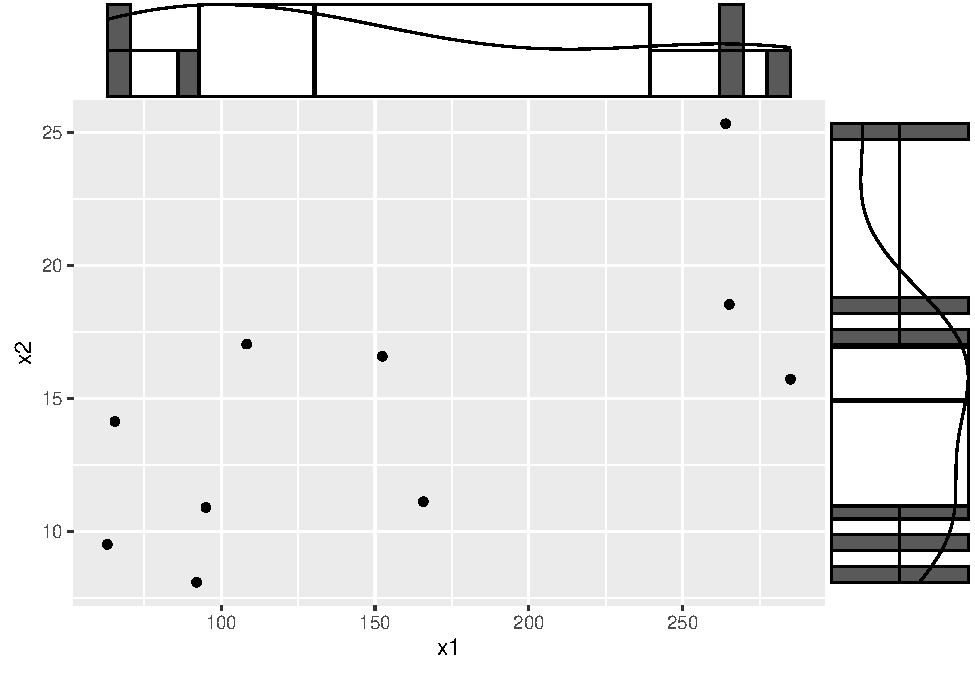
\includegraphics{Tarea1_files/figure-latex/unnamed-chunk-7-1.pdf} Las
ventas tienen mucha variabilidad y no parece seguir una distribución
normal porque se cargan mucho los datos a la izquierda (es difícil tener
ventas grandes). La ganancia parece estar también muy cargada, en
general no se dan ganancias grandes, pero sí aumenta conforme aumentan
las ventas.

\hypertarget{b-1}{%
\subsection{b)}\label{b-1}}

\begin{Shaded}
\begin{Highlighting}[]
\NormalTok{m1 }\OtherTok{\textless{}{-}} \FunctionTok{mean}\NormalTok{(df}\SpecialCharTok{$}\NormalTok{x1)}
\NormalTok{m2 }\OtherTok{\textless{}{-}} \FunctionTok{mean}\NormalTok{(df}\SpecialCharTok{$}\NormalTok{x2)}

\NormalTok{s11 }\OtherTok{\textless{}{-}} \FunctionTok{var}\NormalTok{(df}\SpecialCharTok{$}\NormalTok{x1)}
\NormalTok{s22 }\OtherTok{\textless{}{-}} \FunctionTok{var}\NormalTok{(df}\SpecialCharTok{$}\NormalTok{x2)}

\NormalTok{s12 }\OtherTok{\textless{}{-}} \FunctionTok{cov}\NormalTok{(df}\SpecialCharTok{$}\NormalTok{x1, df}\SpecialCharTok{$}\NormalTok{x2)}
\NormalTok{r12 }\OtherTok{\textless{}{-}} \FunctionTok{cor}\NormalTok{(df}\SpecialCharTok{$}\NormalTok{x1, df}\SpecialCharTok{$}\NormalTok{x2)}

\FunctionTok{cat}\NormalTok{(}\StringTok{"media x1: "}\NormalTok{, m1, }\StringTok{"}\SpecialCharTok{\textbackslash{}n}\StringTok{"}\NormalTok{, }
       \StringTok{"media x2: "}\NormalTok{, m2, }\StringTok{"}\SpecialCharTok{\textbackslash{}n}\StringTok{"}\NormalTok{,}
       \StringTok{"varianza x1: "}\NormalTok{, s11, }\StringTok{"}\SpecialCharTok{\textbackslash{}n}\StringTok{"}\NormalTok{,}
       \StringTok{"varianza x2: "}\NormalTok{, s22, }\StringTok{"}\SpecialCharTok{\textbackslash{}n}\StringTok{"}\NormalTok{,}
       \StringTok{"covarianza: "}\NormalTok{, s12, }\StringTok{"}\SpecialCharTok{\textbackslash{}n}\StringTok{"}\NormalTok{,}
       \StringTok{"correlación: "}\NormalTok{, r12, }\StringTok{"}\SpecialCharTok{\textbackslash{}n}\StringTok{"}\NormalTok{)}
\end{Highlighting}
\end{Shaded}

\begin{verbatim}
media x1:  155.603 
 media x2:  14.704 
 varianza x1:  7476.453 
 varianza x2:  26.19032 
 covarianza:  303.6186 
 correlación:  0.686136 
\end{verbatim}

La correlación no llega a ser fuerte, pero sí hay cierta tendencia entre
ambas variables que nos permite decir que ante un aumento de ventas, hay
un aumento en el profit.

\hypertarget{ejercicio-1.6}{%
\section{Ejercicio 1.6)}\label{ejercicio-1.6}}

\hypertarget{a-2}{%
\subsection{a)}\label{a-2}}

\begin{Shaded}
\begin{Highlighting}[]
\NormalTok{datos }\OtherTok{\textless{}{-}} \FunctionTok{read.table}\NormalTok{(}\StringTok{"data/T1{-}5.DAT"}\NormalTok{, }\AttributeTok{header =} \ConstantTok{FALSE}\NormalTok{)}
\FunctionTok{colnames}\NormalTok{(datos) }\OtherTok{\textless{}{-}} \FunctionTok{c}\NormalTok{(}\StringTok{"Wind"}\NormalTok{, }\StringTok{"Solar\_radiation"}\NormalTok{, }\StringTok{"CO"}\NormalTok{, }\StringTok{"NO"}\NormalTok{, }\StringTok{"NO2"}\NormalTok{, }\StringTok{"O3"}\NormalTok{, }\StringTok{"HC"}\NormalTok{)}

\FunctionTok{pairs}\NormalTok{(datos, }\AttributeTok{pch =} \DecValTok{19}\NormalTok{)}
\end{Highlighting}
\end{Shaded}

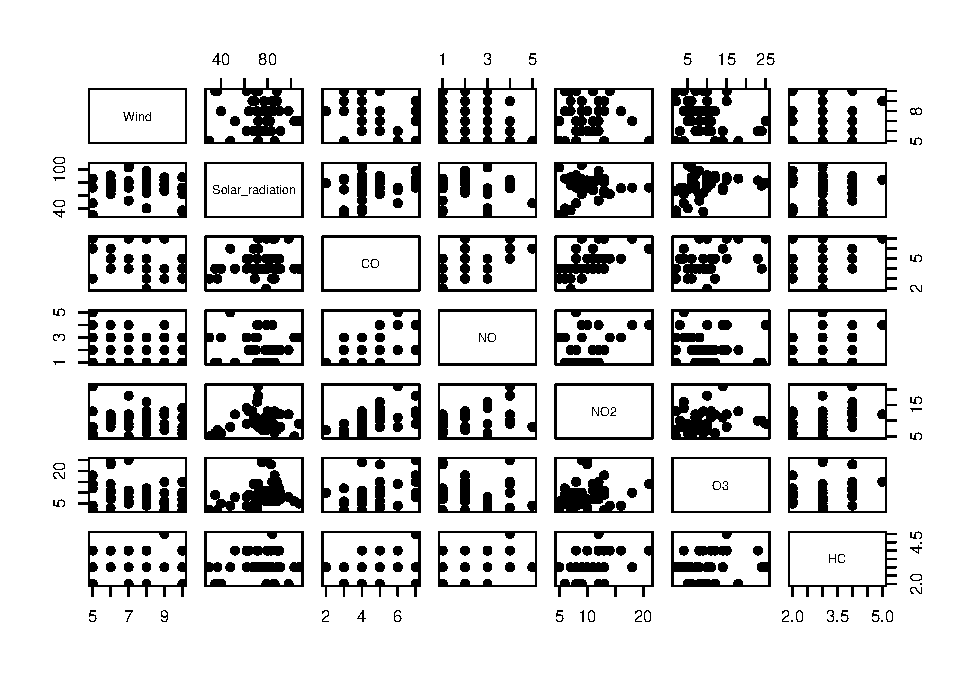
\includegraphics{Tarea1_files/figure-latex/unnamed-chunk-9-1.pdf}

\begin{Shaded}
\begin{Highlighting}[]
\NormalTok{g1 }\OtherTok{\textless{}{-}} \FunctionTok{ggplot}\NormalTok{(datos, }\FunctionTok{aes}\NormalTok{(}\AttributeTok{x =}\NormalTok{ Wind)) }\SpecialCharTok{+}
  \FunctionTok{geom\_histogram}\NormalTok{()}

\NormalTok{g2 }\OtherTok{\textless{}{-}} \FunctionTok{ggplot}\NormalTok{(datos, }\FunctionTok{aes}\NormalTok{(}\AttributeTok{x =}\NormalTok{ Solar\_radiation)) }\SpecialCharTok{+}
  \FunctionTok{geom\_histogram}\NormalTok{()}

\NormalTok{g3 }\OtherTok{\textless{}{-}} \FunctionTok{ggplot}\NormalTok{(datos, }\FunctionTok{aes}\NormalTok{(}\AttributeTok{x =}\NormalTok{ CO)) }\SpecialCharTok{+}
  \FunctionTok{geom\_histogram}\NormalTok{()}

\NormalTok{g4 }\OtherTok{\textless{}{-}} \FunctionTok{ggplot}\NormalTok{(datos, }\FunctionTok{aes}\NormalTok{(}\AttributeTok{x =}\NormalTok{ NO)) }\SpecialCharTok{+}
  \FunctionTok{geom\_histogram}\NormalTok{()}

\NormalTok{g5 }\OtherTok{\textless{}{-}} \FunctionTok{ggplot}\NormalTok{(datos, }\FunctionTok{aes}\NormalTok{(}\AttributeTok{x =}\NormalTok{ NO2)) }\SpecialCharTok{+}
  \FunctionTok{geom\_histogram}\NormalTok{()}

\NormalTok{g6 }\OtherTok{\textless{}{-}} \FunctionTok{ggplot}\NormalTok{(datos, }\FunctionTok{aes}\NormalTok{(}\AttributeTok{x =}\NormalTok{ O3)) }\SpecialCharTok{+}
  \FunctionTok{geom\_histogram}\NormalTok{()}

\NormalTok{g7 }\OtherTok{\textless{}{-}} \FunctionTok{ggplot}\NormalTok{(datos, }\FunctionTok{aes}\NormalTok{(}\AttributeTok{x =}\NormalTok{ HC)) }\SpecialCharTok{+}
  \FunctionTok{geom\_histogram}\NormalTok{()}


\NormalTok{g1}
\end{Highlighting}
\end{Shaded}

\begin{verbatim}
`stat_bin()` using `bins = 30`. Pick better value with `binwidth`.
\end{verbatim}

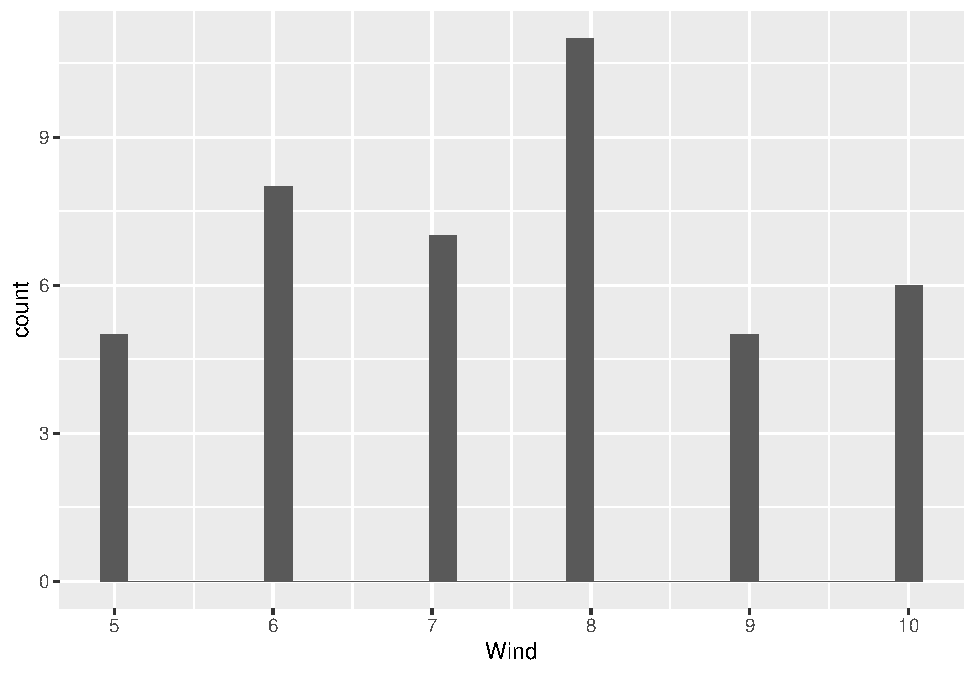
\includegraphics{Tarea1_files/figure-latex/unnamed-chunk-9-2.pdf}

\begin{Shaded}
\begin{Highlighting}[]
\NormalTok{g2}
\end{Highlighting}
\end{Shaded}

\begin{verbatim}
`stat_bin()` using `bins = 30`. Pick better value with `binwidth`.
\end{verbatim}

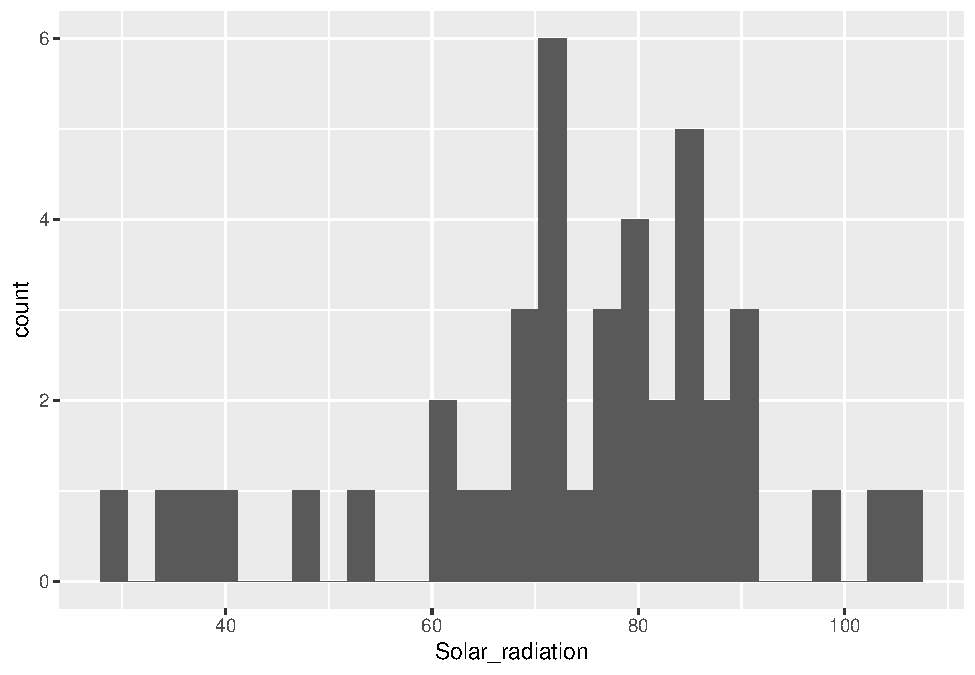
\includegraphics{Tarea1_files/figure-latex/unnamed-chunk-9-3.pdf}

\begin{Shaded}
\begin{Highlighting}[]
\NormalTok{g3}
\end{Highlighting}
\end{Shaded}

\begin{verbatim}
`stat_bin()` using `bins = 30`. Pick better value with `binwidth`.
\end{verbatim}

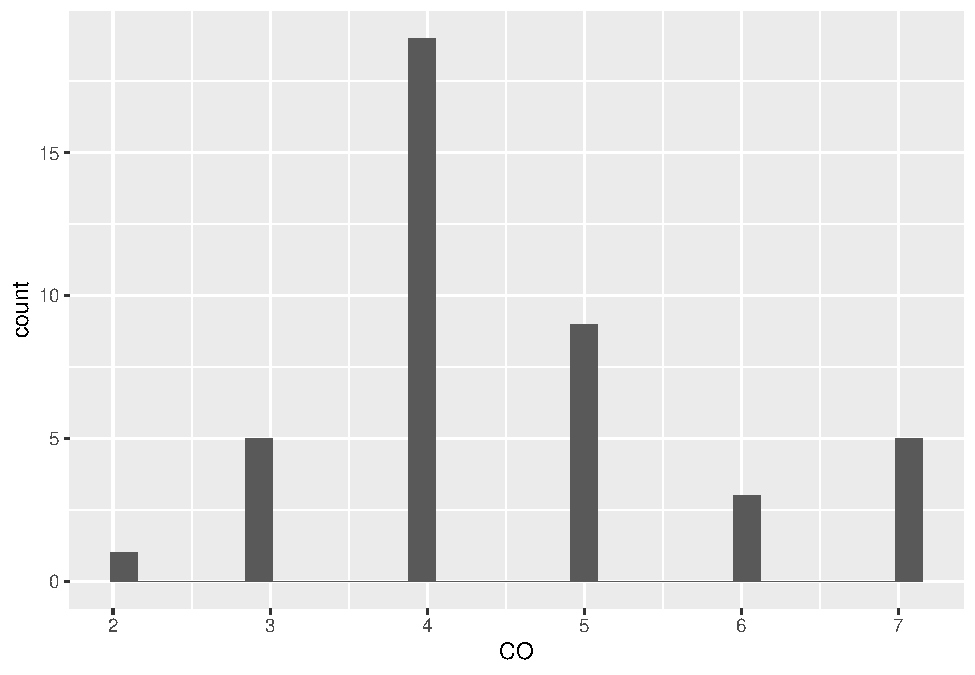
\includegraphics{Tarea1_files/figure-latex/unnamed-chunk-9-4.pdf}

\begin{Shaded}
\begin{Highlighting}[]
\NormalTok{g4}
\end{Highlighting}
\end{Shaded}

\begin{verbatim}
`stat_bin()` using `bins = 30`. Pick better value with `binwidth`.
\end{verbatim}

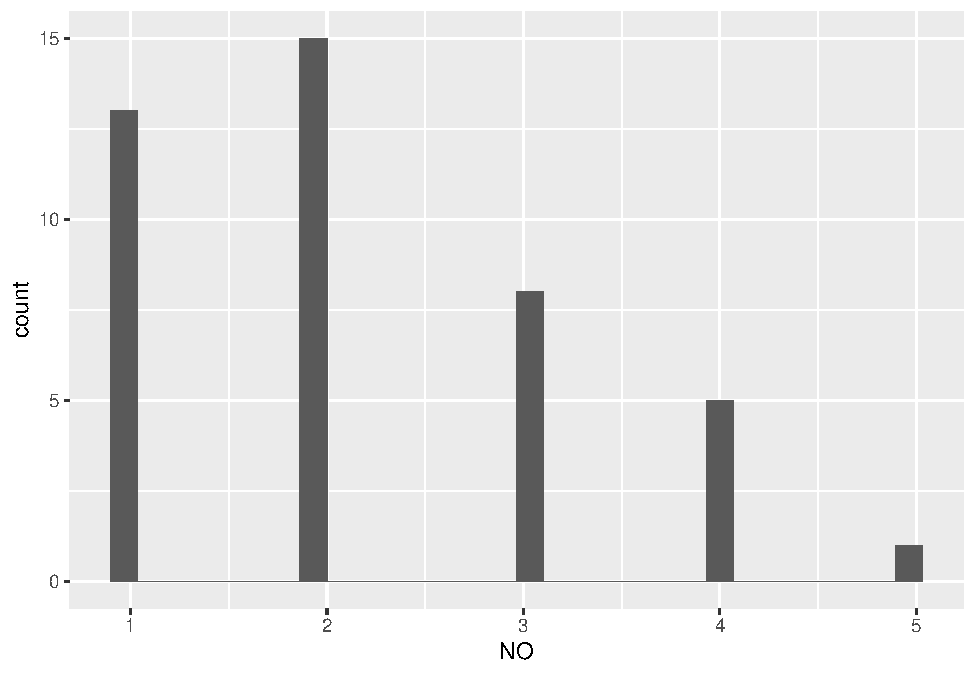
\includegraphics{Tarea1_files/figure-latex/unnamed-chunk-9-5.pdf}

\begin{Shaded}
\begin{Highlighting}[]
\NormalTok{g5}
\end{Highlighting}
\end{Shaded}

\begin{verbatim}
`stat_bin()` using `bins = 30`. Pick better value with `binwidth`.
\end{verbatim}

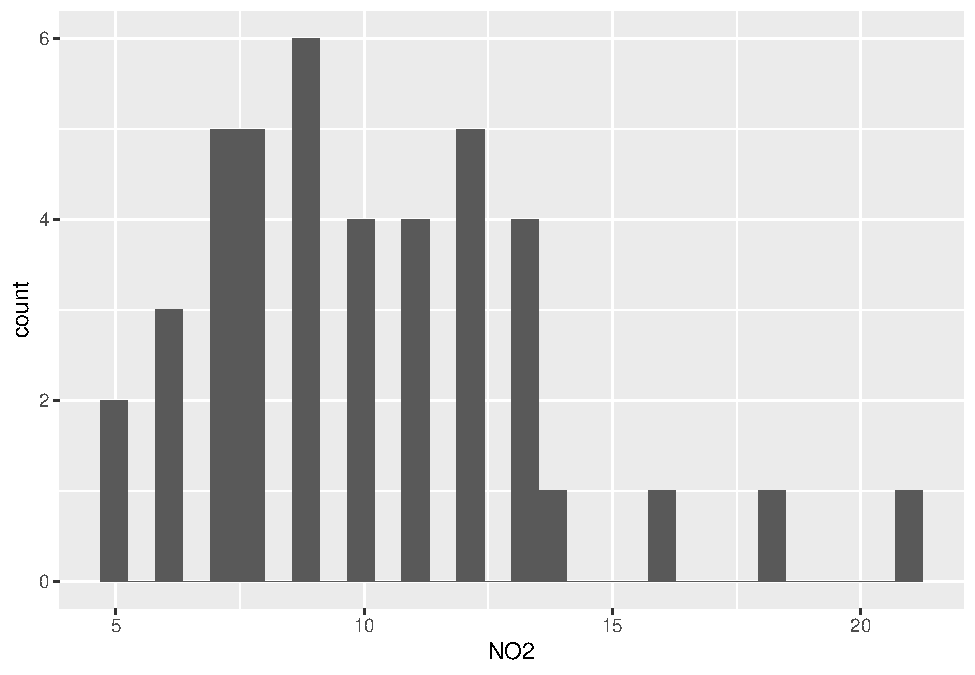
\includegraphics{Tarea1_files/figure-latex/unnamed-chunk-9-6.pdf}

\begin{Shaded}
\begin{Highlighting}[]
\NormalTok{g6}
\end{Highlighting}
\end{Shaded}

\begin{verbatim}
`stat_bin()` using `bins = 30`. Pick better value with `binwidth`.
\end{verbatim}

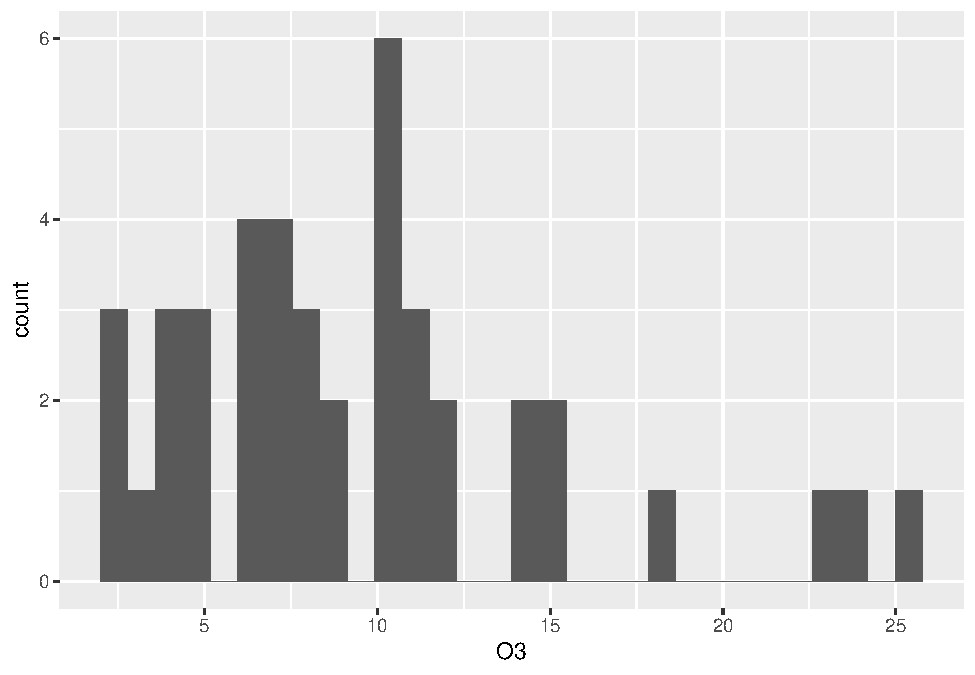
\includegraphics{Tarea1_files/figure-latex/unnamed-chunk-9-7.pdf}

\begin{Shaded}
\begin{Highlighting}[]
\NormalTok{g7}
\end{Highlighting}
\end{Shaded}

\begin{verbatim}
`stat_bin()` using `bins = 30`. Pick better value with `binwidth`.
\end{verbatim}

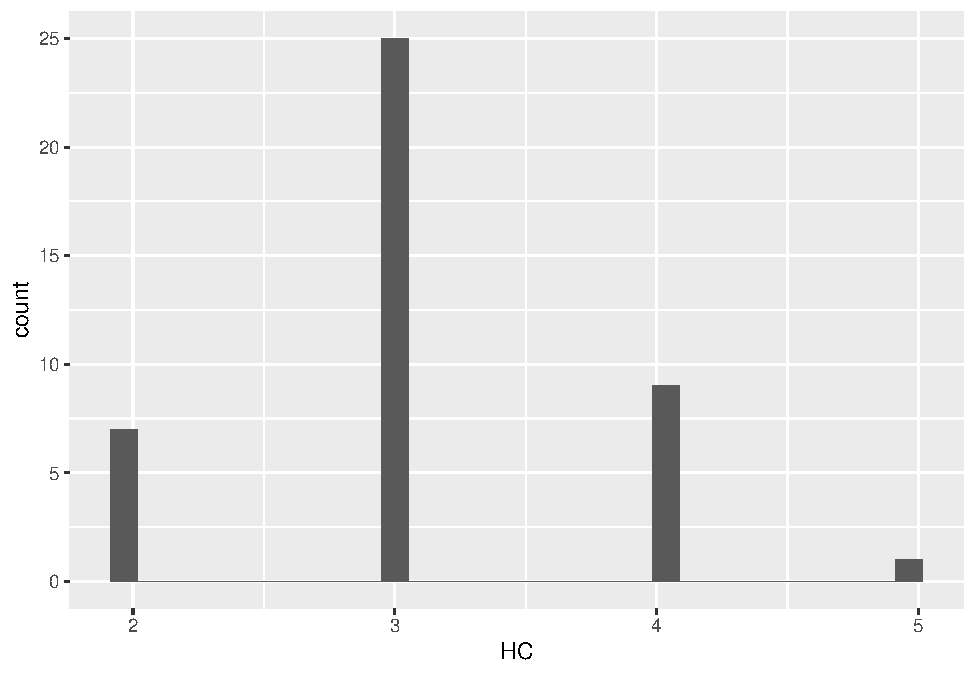
\includegraphics{Tarea1_files/figure-latex/unnamed-chunk-9-8.pdf}

\hypertarget{b-2}{%
\subsection{b)}\label{b-2}}

\begin{Shaded}
\begin{Highlighting}[]
\NormalTok{x }\OtherTok{\textless{}{-}} \FunctionTok{colMeans}\NormalTok{(datos)}
\NormalTok{S }\OtherTok{\textless{}{-}} \FunctionTok{var}\NormalTok{(datos)}
\NormalTok{R }\OtherTok{\textless{}{-}} \FunctionTok{cor}\NormalTok{(datos)}

\NormalTok{x}
\end{Highlighting}
\end{Shaded}

\begin{verbatim}
           Wind Solar_radiation              CO              NO             NO2              O3 
       7.500000       73.857143        4.547619        2.190476       10.047619        9.404762 
             HC 
       3.095238 
\end{verbatim}

\begin{Shaded}
\begin{Highlighting}[]
\NormalTok{S}
\end{Highlighting}
\end{Shaded}

\begin{verbatim}
                      Wind Solar_radiation         CO         NO        NO2         O3        HC
Wind             2.5000000      -2.7804878 -0.3780488 -0.4634146 -0.5853659 -2.2317073 0.1707317
Solar_radiation -2.7804878     300.5156794  3.9094077 -1.3867596  6.7630662 30.7909408 0.6236934
CO              -0.3780488       3.9094077  1.5220674  0.6736353  2.3147503  2.8217189 0.1416957
NO              -0.4634146      -1.3867596  0.6736353  1.1823461  1.0882695 -0.8106852 0.1765389
NO2             -0.5853659       6.7630662  2.3147503  1.0882695 11.3635308  3.1265970 1.0441347
O3              -2.2317073      30.7909408  2.8217189 -0.8106852  3.1265970 30.9785134 0.5946574
HC               0.1707317       0.6236934  0.1416957  0.1765389  1.0441347  0.5946574 0.4785134
\end{verbatim}

\begin{Shaded}
\begin{Highlighting}[]
\NormalTok{R}
\end{Highlighting}
\end{Shaded}

\begin{verbatim}
                      Wind Solar_radiation         CO          NO        NO2         O3         HC
Wind             1.0000000     -0.10144191 -0.1938032 -0.26954261 -0.1098249 -0.2535928 0.15609793
Solar_radiation -0.1014419      1.00000000  0.1827934 -0.07356907  0.1157320  0.3191237 0.05201044
CO              -0.1938032      0.18279338  1.0000000  0.50215246  0.5565838  0.4109288 0.16603235
NO              -0.2695426     -0.07356907  0.5021525  1.00000000  0.2968981 -0.1339521 0.23470432
NO2             -0.1098249      0.11573199  0.5565838  0.29689814  1.0000000  0.1666422 0.44776780
O3              -0.2535928      0.31912373  0.4109288 -0.13395214  0.1666422  1.0000000 0.15445056
HC               0.1560979      0.05201044  0.1660323  0.23470432  0.4477678  0.1544506 1.00000000
\end{verbatim}

Interpretación:

el vector de medias x nos dice el nivel que podemos esperar de cada
medida tomada por el estudio en Los Ángeles, de tal forma que podemos
esperar niveles de CO de 4.54 en un día cualquiera en Los Ángeles.

La matriz S nos permite ver un poco sobre la proporcionalidad entre
pares de mediciones. Si el signo del elemento \$ s\_\{2,1\} \$ es
negativo, como es el caso, podemos observar que las variables
Solar\_radiation y Wind tienen tendencias a ser inversamente
proporcionales. Al contrario si el signo es positivo, podemos argumentar
que hay cierta proporcionalidad o tendencias a ello.

La matriz R nos permite ver la magnitud con la que covarían cierto par
de variables, con esto podemos observar que la relación que tienen las
variables entre ellas no es para nada fuerte, la correlación más fuerte
es 0.55, que pertenece al par de variables (NO2, CO).

\hypertarget{ejercicio-1.8}{%
\section{Ejercicio 1.8}\label{ejercicio-1.8}}

\hypertarget{a-3}{%
\subsection{a)}\label{a-3}}

\(Dado\left(P,Q\right)=\sqrt{\left(x_1-y_1\right)^2+\ldots+\left(x_p-y_p\right)^2}\ y\ P=\left(-1,-1\right)Q=\left(1,0\right)\)

\(\rightarrow\ d\left(P,Q\right)=\sqrt{\left(-1-1\right)^2+\left(-1-0\right)^2}=\sqrt{\left(-2\right)^2+\left(-1\right)^2}=\sqrt{4+1}=\sqrt5\)

\hypertarget{b-3}{%
\subsection{b)}\label{b-3}}

\(Dado\ d\left(P,Q\right)=\sqrt{a_{11}\left(x_1-y_1\right)^2+2a_{12}\left(x_1-y_1\right)\left(x_2-y_2\right)+{a_{22}\left(x_2-y_2\right)}^2}\)
\(P=\left(-1,-1\right)\ Q=\left(1,0\right)\ \ a_{11}=\frac{1}{3}\ \ a_{22}=\frac{4}{27}\ \ a_{12}=\frac{1}{9}\)
\(\sqrt{{\frac{1}{3}\left(-1-1\right)}^2+\frac{4}{27}\left(-1-0\right)^2+\left(-1-1\right)\left(-1-0\right)\frac{1}{9}}\)
\(=\sqrt{\frac{4}{3}+\frac{4}{27}+\frac{2}{9}}=\sqrt{\frac{36+4+6}{27}}=\sqrt{\frac{46}{27}}\)

\hypertarget{c-1}{%
\subsection{c)}\label{c-1}}

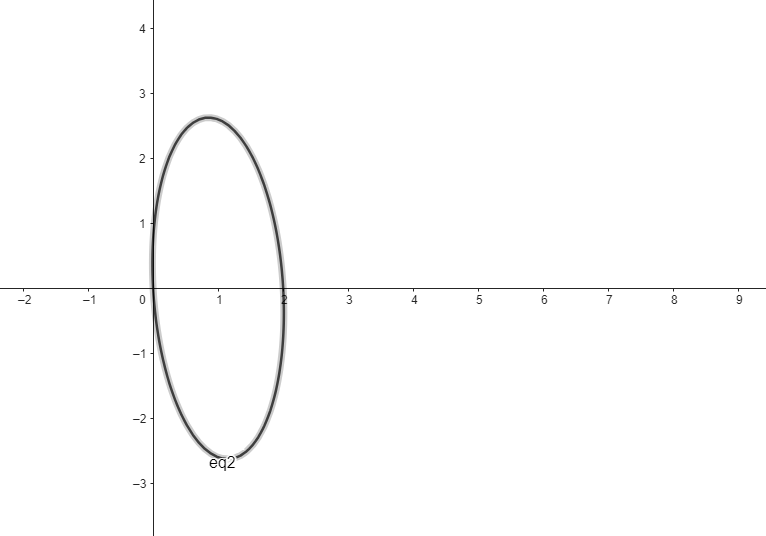
\includegraphics{assets/distancia1.png}

\hypertarget{ejercicio-1.10}{%
\section{Ejercicio 1.10}\label{ejercicio-1.10}}

\(Para\ que\ una\ función\ sea\ considerada\ una\ metrica\ se\ deben\ de\ cumplir\ las\ siguientes\ propiedades:\)

\(d\left(x,y\right)\geq0\)

\(d\left(x,y\right)=d\left(y,x\right)\)

\(d\left(x,z\right)\le\ d\left(x,y\right)+d\left(y,z\right)\)

\(d\left(x,y\right)=0\ \ sii\ \ \ x=y\)

\hypertarget{a-4}{%
\subsection{a)}\label{a-4}}

\(Para\ d\left(P\right)=x_1^2+4x_2^2+x_2x_1\)

\(No\ se\ cumple,ya\ que\ para\ p=\left(1,3\right)\ y\ q=\left(3,1\right)\ d\left(x,y\right)\neq\ d\left(y,x\right)\)

\(1+4\ast9+3=9+4+3\rightarrow40=16\ \ \ !\)

\hypertarget{b-4}{%
\subsection{b)}\label{b-4}}

\(Para\ d(P)=x^2_1-2x_2^2\ \)

\(No\ se\ cumple,ya\ que\ para\ p=\left(1,3\right)\ \ d\left(x,y\right)<0\)

\(1-2\ast9<=0 \  ->\  -17>=0\ !\)

\hypertarget{ejercicio-1.12}{%
\section{Ejercicio 1.12}\label{ejercicio-1.12}}

\hypertarget{a-5}{%
\subsection{a)}\label{a-5}}

\(Sea\ d\left(O,P\right)=\max{\left(\left|x_1\right|,\left|x_2\right|\right)}\)

\(Para\ P=\left(-3,4\right)=\max{\left(\left|-3\right|,\left|4\right|\right)}=\max{\left(3,4\right)}=4\)

\hypertarget{b-5}{%
\subsection{b)}\label{b-5}}

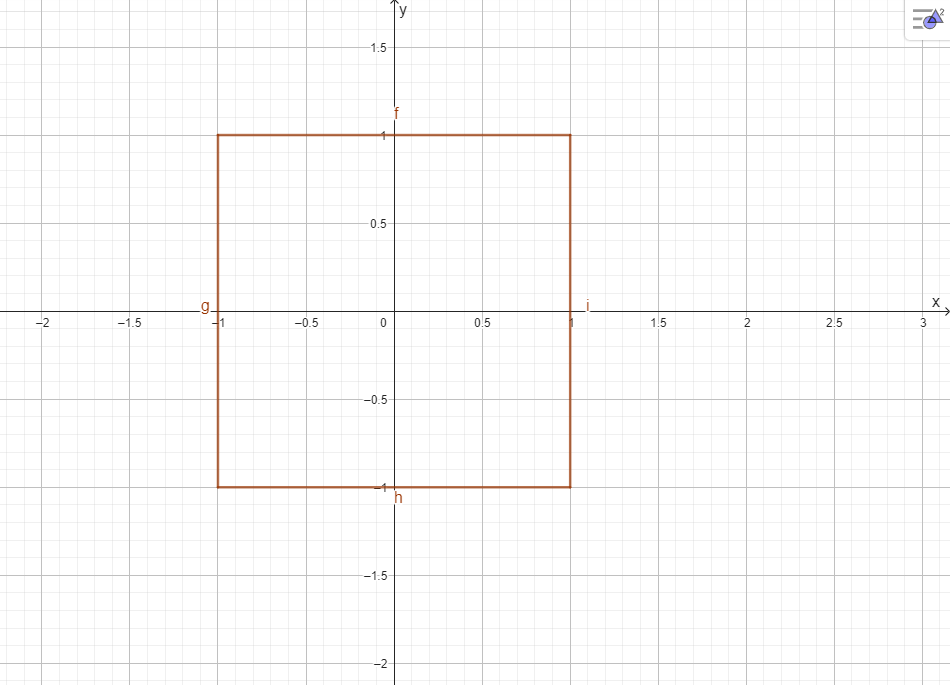
\includegraphics{puntosDisntancia1maxAbs.png}

\hypertarget{c-2}{%
\subsection{c)}\label{c-2}}

\(Basandonos\ en\ la\ expresión\ original,\ podemos\ generalizar\ la\ expresión\ a\ p\ dimensiones\ de\ \)

\(\mathrm{la\ siguiente\ manera\ d}\left(\mathrm{P,O}\right)\mathrm{\mathrm{=}}\mathrm{max}{\left(\left|\mathrm{x}_\mathrm{1}\right|\mathrm{,} \left|\mathrm{x}_\mathrm{2}\right|\mathrm{,\ldots,} \left|\mathrm{x}_\mathrm{p}\right|\right)}\)

\hypertarget{ejercicio-1.14}{%
\section{Ejercicio 1.14}\label{ejercicio-1.14}}

\hypertarget{a-6}{%
\subsection{a)}\label{a-6}}

\begin{verbatim}
`geom_smooth()` using formula = 'y ~ x'
\end{verbatim}

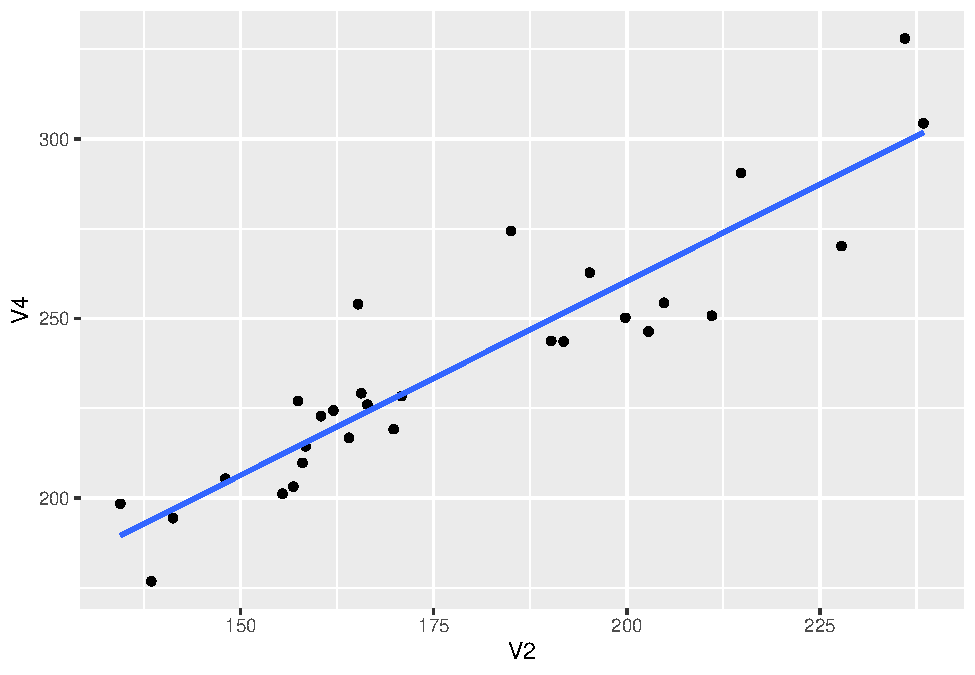
\includegraphics{Tarea1_files/figure-latex/pressure-1.pdf}

Paceriera seguir un comportamiento lineal con correalación positiva, ya
que al ajustar una regresión lineal a este conjunto de datos podemos ver
de mejor manera esta posible relación.

\hypertarget{b-6}{%
\subsection{b)}\label{b-6}}

Medias para ambas clases

\begin{longtable}[]{@{}
  >{\centering\arraybackslash}p{(\columnwidth - 10\tabcolsep) * \real{0.2083}}
  >{\centering\arraybackslash}p{(\columnwidth - 10\tabcolsep) * \real{0.1111}}
  >{\centering\arraybackslash}p{(\columnwidth - 10\tabcolsep) * \real{0.1111}}
  >{\centering\arraybackslash}p{(\columnwidth - 10\tabcolsep) * \real{0.1111}}
  >{\centering\arraybackslash}p{(\columnwidth - 10\tabcolsep) * \real{0.1111}}
  >{\centering\arraybackslash}p{(\columnwidth - 10\tabcolsep) * \real{0.1111}}@{}}
\toprule()
\begin{minipage}[b]{\linewidth}\centering
Group.1
\end{minipage} & \begin{minipage}[b]{\linewidth}\centering
V1
\end{minipage} & \begin{minipage}[b]{\linewidth}\centering
V2
\end{minipage} & \begin{minipage}[b]{\linewidth}\centering
V3
\end{minipage} & \begin{minipage}[b]{\linewidth}\centering
V4
\end{minipage} & \begin{minipage}[b]{\linewidth}\centering
V5
\end{minipage} \\
\midrule()
\endhead
Non-Positive & 37.99 & 147.3 & 1.562 & 195.6 & 1.62 \\
Positive & 42.07 & 178.3 & 12.28 & 236.9 & 13.08 \\
\bottomrule()
\end{longtable}

Para esclerosis esto resulta \(S_n\)

\begin{longtable}[]{@{}
  >{\centering\arraybackslash}p{(\columnwidth - 10\tabcolsep) * \real{0.1250}}
  >{\centering\arraybackslash}p{(\columnwidth - 10\tabcolsep) * \real{0.1250}}
  >{\centering\arraybackslash}p{(\columnwidth - 10\tabcolsep) * \real{0.1111}}
  >{\centering\arraybackslash}p{(\columnwidth - 10\tabcolsep) * \real{0.1250}}
  >{\centering\arraybackslash}p{(\columnwidth - 10\tabcolsep) * \real{0.1111}}
  >{\centering\arraybackslash}p{(\columnwidth - 10\tabcolsep) * \real{0.1250}}@{}}
\toprule()
\begin{minipage}[b]{\linewidth}\centering
~
\end{minipage} & \begin{minipage}[b]{\linewidth}\centering
V1
\end{minipage} & \begin{minipage}[b]{\linewidth}\centering
V2
\end{minipage} & \begin{minipage}[b]{\linewidth}\centering
V3
\end{minipage} & \begin{minipage}[b]{\linewidth}\centering
V4
\end{minipage} & \begin{minipage}[b]{\linewidth}\centering
V5
\end{minipage} \\
\midrule()
\endhead
\textbf{V1} & 117 & 50.97 & -19.52 & 65.78 & -28.79 \\
\textbf{V2} & 50.97 & 815.6 & 236 & 881 & 103.1 \\
\textbf{V3} & -19.52 & 236 & 306.3 & 224.4 & 287.1 \\
\textbf{V4} & 65.78 & 881 & 224.4 & 1139 & 78.3 \\
\textbf{V5} & -28.79 & 103.1 & 287.1 & 78.3 & 338.9 \\
\bottomrule()
\end{longtable}

Para no esclerosis esto resulta \(S_n\)

\begin{longtable}[]{@{}
  >{\centering\arraybackslash}p{(\columnwidth - 10\tabcolsep) * \real{0.1250}}
  >{\centering\arraybackslash}p{(\columnwidth - 10\tabcolsep) * \real{0.1111}}
  >{\centering\arraybackslash}p{(\columnwidth - 10\tabcolsep) * \real{0.1111}}
  >{\centering\arraybackslash}p{(\columnwidth - 10\tabcolsep) * \real{0.1250}}
  >{\centering\arraybackslash}p{(\columnwidth - 10\tabcolsep) * \real{0.1111}}
  >{\centering\arraybackslash}p{(\columnwidth - 10\tabcolsep) * \real{0.1250}}@{}}
\toprule()
\begin{minipage}[b]{\linewidth}\centering
~
\end{minipage} & \begin{minipage}[b]{\linewidth}\centering
V1
\end{minipage} & \begin{minipage}[b]{\linewidth}\centering
V2
\end{minipage} & \begin{minipage}[b]{\linewidth}\centering
V3
\end{minipage} & \begin{minipage}[b]{\linewidth}\centering
V4
\end{minipage} & \begin{minipage}[b]{\linewidth}\centering
V5
\end{minipage} \\
\midrule()
\endhead
\textbf{V1} & 273.6 & 94.02 & 5.284 & 102.2 & 3.194 \\
\textbf{V2} & 94.02 & 110.7 & 1.741 & 105.2 & 2.013 \\
\textbf{V3} & 5.284 & 1.741 & 1.779 & 2.202 & 0.4941 \\
\textbf{V4} & 102.2 & 105.2 & 2.202 & 182.5 & 2.317 \\
\textbf{V5} & 3.194 & 2.013 & 0.4941 & 2.317 & 2.321 \\
\bottomrule()
\end{longtable}

Para esclerosis esta es la matriz R

\begin{longtable}[]{@{}
  >{\centering\arraybackslash}p{(\columnwidth - 10\tabcolsep) * \real{0.1250}}
  >{\centering\arraybackslash}p{(\columnwidth - 10\tabcolsep) * \real{0.1389}}
  >{\centering\arraybackslash}p{(\columnwidth - 10\tabcolsep) * \real{0.1250}}
  >{\centering\arraybackslash}p{(\columnwidth - 10\tabcolsep) * \real{0.1389}}
  >{\centering\arraybackslash}p{(\columnwidth - 10\tabcolsep) * \real{0.1250}}
  >{\centering\arraybackslash}p{(\columnwidth - 10\tabcolsep) * \real{0.1389}}@{}}
\toprule()
\begin{minipage}[b]{\linewidth}\centering
~
\end{minipage} & \begin{minipage}[b]{\linewidth}\centering
V1
\end{minipage} & \begin{minipage}[b]{\linewidth}\centering
V2
\end{minipage} & \begin{minipage}[b]{\linewidth}\centering
V3
\end{minipage} & \begin{minipage}[b]{\linewidth}\centering
V4
\end{minipage} & \begin{minipage}[b]{\linewidth}\centering
V5
\end{minipage} \\
\midrule()
\endhead
\textbf{V1} & 1 & 0.165 & -0.1031 & 0.1802 & -0.1446 \\
\textbf{V2} & 0.165 & 1 & 0.4722 & 0.9139 & 0.1961 \\
\textbf{V3} & -0.1031 & 0.4722 & 1 & 0.3798 & 0.8909 \\
\textbf{V4} & 0.1802 & 0.9139 & 0.3798 & 1 & 0.126 \\
\textbf{V5} & -0.1446 & 0.1961 & 0.8909 & 0.126 & 1 \\
\bottomrule()
\end{longtable}

Para no esclerosis esta es la matriz R

\begin{longtable}[]{@{}
  >{\centering\arraybackslash}p{(\columnwidth - 10\tabcolsep) * \real{0.1250}}
  >{\centering\arraybackslash}p{(\columnwidth - 10\tabcolsep) * \real{0.1250}}
  >{\centering\arraybackslash}p{(\columnwidth - 10\tabcolsep) * \real{0.1250}}
  >{\centering\arraybackslash}p{(\columnwidth - 10\tabcolsep) * \real{0.1250}}
  >{\centering\arraybackslash}p{(\columnwidth - 10\tabcolsep) * \real{0.1250}}
  >{\centering\arraybackslash}p{(\columnwidth - 10\tabcolsep) * \real{0.1250}}@{}}
\toprule()
\begin{minipage}[b]{\linewidth}\centering
~
\end{minipage} & \begin{minipage}[b]{\linewidth}\centering
V1
\end{minipage} & \begin{minipage}[b]{\linewidth}\centering
V2
\end{minipage} & \begin{minipage}[b]{\linewidth}\centering
V3
\end{minipage} & \begin{minipage}[b]{\linewidth}\centering
V4
\end{minipage} & \begin{minipage}[b]{\linewidth}\centering
V5
\end{minipage} \\
\midrule()
\endhead
\textbf{V1} & 1 & 0.5403 & 0.2395 & 0.4574 & 0.1268 \\
\textbf{V2} & 0.5403 & 1 & 0.1241 & 0.7404 & 0.1256 \\
\textbf{V3} & 0.2395 & 0.1241 & 1 & 0.1222 & 0.2431 \\
\textbf{V4} & 0.4574 & 0.7404 & 0.1222 & 1 & 0.1126 \\
\textbf{V5} & 0.1268 & 0.1256 & 0.2431 & 0.1126 & 1 \\
\bottomrule()
\end{longtable}

\hypertarget{ejercicio-1.16}{%
\section{Ejercicio 1.16}\label{ejercicio-1.16}}

Falta

\hypertarget{ejercicio-1.18}{%
\section{Ejercicio 1.18}\label{ejercicio-1.18}}

Convertir los datos de la tabla a rapidez medida en m/s. Calcular
\(\bar{x}\),\(S_n\), \(R\). Interpretar las correlaciones a pares.

\begin{Shaded}
\begin{Highlighting}[]
\NormalTok{datos }\OtherTok{\textless{}{-}} \FunctionTok{read.table}\NormalTok{(}\StringTok{"data/T1{-}9.DAT"}\NormalTok{)}

\NormalTok{datos }\OtherTok{\textless{}{-}}\NormalTok{ datos }\SpecialCharTok{\%\textgreater{}\%} \FunctionTok{mutate}\NormalTok{(}\AttributeTok{speed\_100 =} \DecValTok{100} \SpecialCharTok{/}\NormalTok{ V1, }\AttributeTok{speed\_200 =} \DecValTok{200} \SpecialCharTok{/}\NormalTok{ V2,}
\AttributeTok{speed\_400 =} \DecValTok{400} \SpecialCharTok{/}\NormalTok{ V3, }\AttributeTok{speed\_800 =} \DecValTok{800} \SpecialCharTok{/}\NormalTok{ (V4 }\SpecialCharTok{*} \DecValTok{60}\NormalTok{),}
\AttributeTok{speed\_1500 =} \DecValTok{1500} \SpecialCharTok{/}\NormalTok{ (V5 }\SpecialCharTok{*} \DecValTok{60}\NormalTok{), }\AttributeTok{speed\_3000 =} \DecValTok{3000} \SpecialCharTok{/}\NormalTok{ (V6 }\SpecialCharTok{*} \DecValTok{60}\NormalTok{),}
\AttributeTok{speed\_marathon =} \DecValTok{42195} \SpecialCharTok{/}\NormalTok{ (V7 }\SpecialCharTok{*} \DecValTok{60}\NormalTok{))}
\NormalTok{X }\OtherTok{\textless{}{-}}\NormalTok{ datos }\SpecialCharTok{\%\textgreater{}\%} \FunctionTok{select}\NormalTok{(speed\_100, speed\_200, speed\_400,}
\NormalTok{speed\_800, speed\_1500, speed\_3000, speed\_marathon)}
\end{Highlighting}
\end{Shaded}

Vector de medias

\begin{Shaded}
\begin{Highlighting}[]
\NormalTok{x\_bar }\OtherTok{\textless{}{-}} \FunctionTok{colMeans}\NormalTok{(X)}
\NormalTok{x\_bar}
\end{Highlighting}
\end{Shaded}

\begin{verbatim}
     speed_100      speed_200      speed_400      speed_800     speed_1500     speed_3000 
      8.619563       8.477682       7.508260       6.438315       5.809894       5.327651 
speed_marathon 
      4.154344 
\end{verbatim}

Matriz de covarianza

\begin{Shaded}
\begin{Highlighting}[]
\NormalTok{n }\OtherTok{\textless{}{-}} \FunctionTok{nrow}\NormalTok{(X)}
\NormalTok{S }\OtherTok{\textless{}{-}} \FunctionTok{var}\NormalTok{(X)}
\NormalTok{Sn }\OtherTok{\textless{}{-}}\NormalTok{ (n}\DecValTok{{-}1}\NormalTok{)}\SpecialCharTok{/}\NormalTok{n }\SpecialCharTok{*}\NormalTok{ S}
\NormalTok{Sn}
\end{Highlighting}
\end{Shaded}

\begin{verbatim}
                speed_100  speed_200 speed_400  speed_800 speed_1500 speed_3000 speed_marathon
speed_100      0.10760676 0.12153268 0.1020016 0.07809972 0.09734084  0.1013165      0.1323820
speed_200      0.12153268 0.15053074 0.1241922 0.09227774 0.11161663  0.1152740      0.1553819
speed_400      0.10200163 0.12419217 0.1382760 0.10913176 0.11949475  0.1200003      0.1490451
speed_800      0.07809972 0.09227774 0.1091318 0.10656842 0.11982963  0.1177373      0.1441559
speed_1500     0.09734084 0.11161663 0.1194947 0.11982963 0.15951532  0.1588241      0.1928020
speed_3000     0.10131654 0.11527402 0.1200003 0.11773734 0.15882406  0.1702817      0.2059045
speed_marathon 0.13238201 0.15538191 0.1490451 0.14415595 0.19280198  0.2059045      0.3157511
\end{verbatim}

Matriz de correlaciones

\begin{Shaded}
\begin{Highlighting}[]
\NormalTok{R }\OtherTok{\textless{}{-}} \FunctionTok{cor}\NormalTok{(X)}
\NormalTok{R}
\end{Highlighting}
\end{Shaded}

\begin{verbatim}
               speed_100 speed_200 speed_400 speed_800 speed_1500 speed_3000 speed_marathon
speed_100      1.0000000 0.9549062 0.8362072 0.7293155  0.7429749  0.7484738      0.7181856
speed_200      0.9549062 1.0000000 0.8608117 0.7285680  0.7203028  0.7200039      0.7127142
speed_400      0.8362072 0.8608117 1.0000000 0.8990078  0.8045891  0.7820324      0.7132994
speed_800      0.7293155 0.7285680 0.8990078 1.0000000  0.9190704  0.8740091      0.7858612
speed_1500     0.7429749 0.7203028 0.8045891 0.9190704  1.0000000  0.9636761      0.8590883
speed_3000     0.7484738 0.7200039 0.7820324 0.8740091  0.9636761  1.0000000      0.8879928
speed_marathon 0.7181856 0.7127142 0.7132994 0.7858612  0.8590883  0.8879928      1.0000000
\end{verbatim}

Se puede observar que todas las correlaciones entre los valores de
rapidez son positivas. Se puede observar que después del valor 1 de la
diagonal principal, las correlaciones tienden a disminuir y antes del
valor tienden a aumentar. Cuando la disntancia aumenta el tiempo en
completarlo también aumenta, pero naturalmente, la rapidez promedio para
completar un maratón es menor que la de un circuito de 100 m.

\hypertarget{ejercicio-1.20}{%
\section{Ejercicio 1.20}\label{ejercicio-1.20}}

\begin{verbatim}
No trace type specified:
  Based on info supplied, a 'scatter3d' trace seems appropriate.
  Read more about this trace type -> https://plotly.com/r/reference/#scatter3d
\end{verbatim}

\begin{verbatim}
No scatter3d mode specifed:
  Setting the mode to markers
  Read more about this attribute -> https://plotly.com/r/reference/#scatter-mode
\end{verbatim}

\begin{verbatim}
PhantomJS not found. You can install it with webshot::install_phantomjs(). If it is installed, please make sure the phantomjs executable can be found via the PATH variable.
\end{verbatim}

\begin{verbatim}
NULL
\end{verbatim}

Se puede observar que una gran cantidad de puntos se concentran en un
cúmulo alrededor del (-0.2, 0.4) en el eje x, (-0.2, 0.2) en el eje y,
(1, 3.27) en el eje z. El punto con las coordenadas (0.58, 0.04, 5.06)
parece ser un dato atípico. b) Colorear los puntos de acuerdo a los que
están en bancarrota ¿Hay alguna orientación en la que se pueden
distinguir las compañías en bancarrota de las que no lo están? ¿Existen
observaciones que pueden llegar a tener un impacto significativo en
alguna regla para clasicar nuevas empresas?

\begin{Shaded}
\begin{Highlighting}[]
\NormalTok{datos}\SpecialCharTok{$}\NormalTok{V5 }\OtherTok{\textless{}{-}} \FunctionTok{as.factor}\NormalTok{(datos}\SpecialCharTok{$}\NormalTok{V5)}

\CommentTok{\#fig \textless{}{-} plot\_ly(datos, x = \textasciitilde{}V1, y = \textasciitilde{}V2, z = \textasciitilde{}V3, color = \textasciitilde{}V5,}
\CommentTok{\#colors = c("\#FF0000", "\#0000FF"))}
\CommentTok{\#fig}
\end{Highlighting}
\end{Shaded}

Si orientamos el eje X con x2, el eje y con x3 y el eje z con x1 se
puede disntiguir a una gran mayoría de las compañías en bancarrota,
específicamente, las que están en bancarrota tienden a tener menor x2,
menor x3 y menor x1. En las empresas que no están en bancarrota un punto
que puede tener un gran impacto puede ser el (0.14, -0.03, 0.46) debido
a que presenta un valor de x3 muy bajo. En el caso de las que sí están
en bancarrota podría ser el (0.37, 0.11, 1.99) debido a su valor mayor
de x1.

\hypertarget{ejercicio-1.22}{%
\section{Ejercicio 1.22}\label{ejercicio-1.22}}

\begin{Shaded}
\begin{Highlighting}[]
\NormalTok{datos }\OtherTok{\textless{}{-}} \FunctionTok{read.table}\NormalTok{(}\StringTok{"data/T6{-}12.DAT"}\NormalTok{) }\SpecialCharTok{\%\textgreater{}\%} \FunctionTok{select}\NormalTok{(V1, V2, V3, V4)}
\end{Highlighting}
\end{Shaded}

\begin{Shaded}
\begin{Highlighting}[]
\NormalTok{x\_bar }\OtherTok{\textless{}{-}} \FunctionTok{colMeans}\NormalTok{(datos)}
\NormalTok{x\_bar}
\end{Highlighting}
\end{Shaded}

\begin{verbatim}
     V1      V2      V3      V4 
 0.3554  5.2542  3.0014 43.7876 
\end{verbatim}

\hypertarget{a-graficar-el-dataset-en-3-dimensiones.}{%
\subsection{a) Graficar el dataset en 3
dimensiones.}\label{a-graficar-el-dataset-en-3-dimensiones.}}

\begin{Shaded}
\begin{Highlighting}[]
\CommentTok{\#fig \textless{}{-} plot\_ly(datos, x = \textasciitilde{}V1, y = \textasciitilde{}V2, z = \textasciitilde{}V3)}
\CommentTok{\#fig}
\end{Highlighting}
\end{Shaded}

\hypertarget{b-checar-outliers.}{%
\subsection{b) Checar outliers.}\label{b-checar-outliers.}}

Un valor que parece ser un outlier es el (-0.45, -0.41, 1.09) ya que sus
valores en las tres coordendas son menores que la media.

\hypertarget{ejercicio-1.24}{%
\section{Ejercicio 1.24}\label{ejercicio-1.24}}

Representar el dataset con caras de Chernoff ¿Existen diferentes grupos?

\begin{Shaded}
\begin{Highlighting}[]
\NormalTok{datos }\OtherTok{\textless{}{-}} \FunctionTok{read.table}\NormalTok{(}\StringTok{"data/T12{-}4.DAT"}\NormalTok{) }\SpecialCharTok{\%\textgreater{}\%} \FunctionTok{select}\NormalTok{(V1, V2, V3, V4, V5, V6, V7, V8)}

\FunctionTok{faces}\NormalTok{(datos, }\AttributeTok{face.type =} \DecValTok{1}\NormalTok{)}
\end{Highlighting}
\end{Shaded}

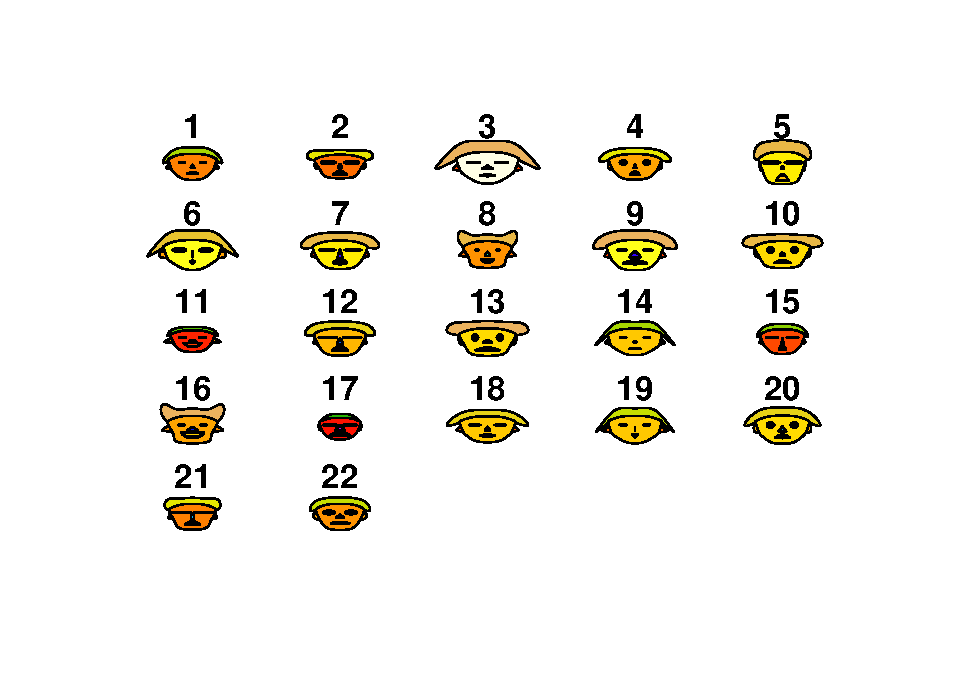
\includegraphics{Tarea1_files/figure-latex/unnamed-chunk-26-1.pdf}

\begin{verbatim}
effect of variables:
 modified item       Var 
 "height of face   " "V1"
 "width of face    " "V2"
 "structure of face" "V3"
 "height of mouth  " "V4"
 "width of mouth   " "V5"
 "smiling          " "V6"
 "height of eyes   " "V7"
 "width of eyes    " "V8"
 "height of hair   " "V1"
 "width of hair   "  "V2"
 "style of hair   "  "V3"
 "height of nose  "  "V4"
 "width of nose   "  "V5"
 "width of ear    "  "V6"
 "height of ear   "  "V7"
\end{verbatim}

Existen algunas compañías que sus representaciones se parecen, por
ejemplo, la 7, 9, 12 y la 11, 15, 17.

\hypertarget{ejercicio-1.26}{%
\section{Ejercicio 1.26}\label{ejercicio-1.26}}

\end{document}
